\section*{Table des annexe}
\addcontentsline{toc}{section}{Annexe}

% Pour créer une table des matières des annexes
\newcommand{\listappendicesname}{}
\newlistof{appendices}{apc}{\listappendicesname}
\newcommand{\appendices}[1]{\addcontentsline{apc}{appendices}{#1}}
\newcommand{\newappendix}[1]{\section{#1}\appendices{#1}}
\parindent0mm

\listofappendices
\addtocontents{toc}{\protect\setcounter{tocdepth}{-1}} %Pour pas afficher les annexe dans la table des matières principales
\newpage
\thispagestyle{empty} % Supprime les numéros de page et l'en-tête de cette page
\mbox{} % Ajoute un espace vide pour remplir la page blanche
\newpage

\newappendix{Connecting the dots, réseau complet}
\label{an:modelling_full}
\begin{figure}[ht]
\centering
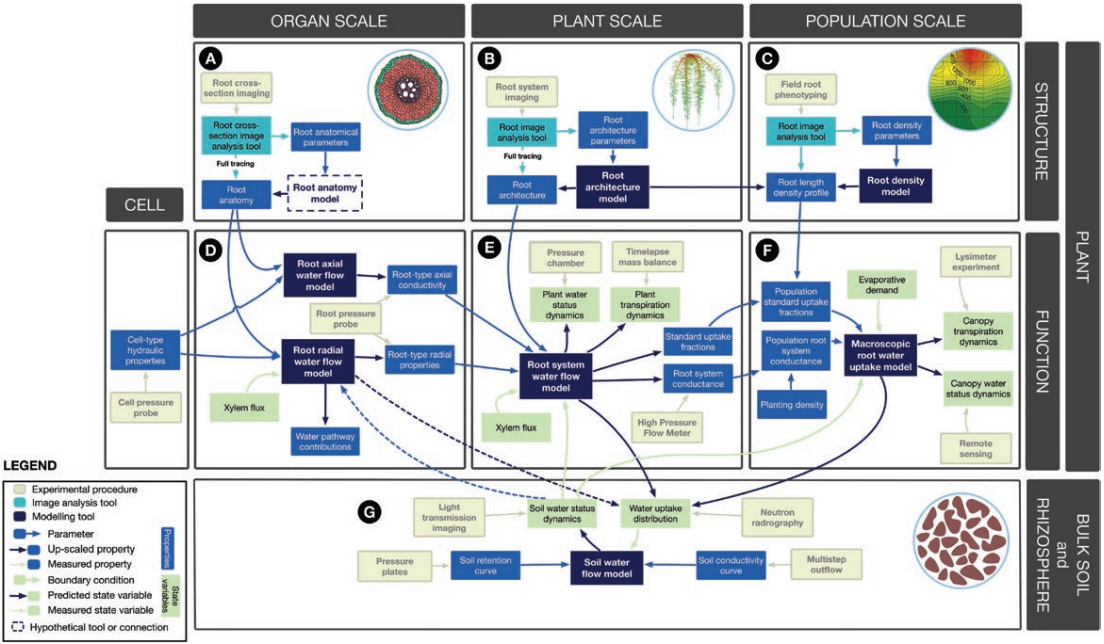
\includegraphics[width=1\textwidth]{Image/modelling.png}
\caption{Réseau complet de \cite{passot_connecting_2018}}
\end{figure}

\newpage

\newappendix{Configuration du scanner}
\label{an:config}
\begin{figure}[ht]
\centering
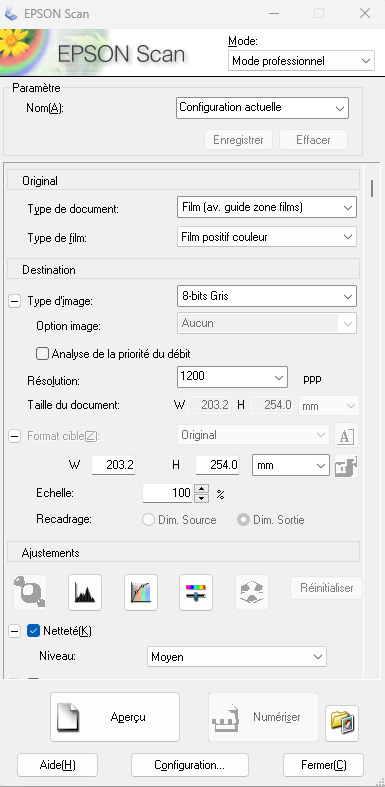
\includegraphics[width=0.5\textwidth]{Image/config scanner.png}
\caption{Configuration utilisée pour numériser les échantillons racinaire}
\end{figure}

\newpage

\newappendix{Protocole des tests de culture du CIPF}
\label{an:protocole_CIPF}
\begin{figure}[ht]
\centering
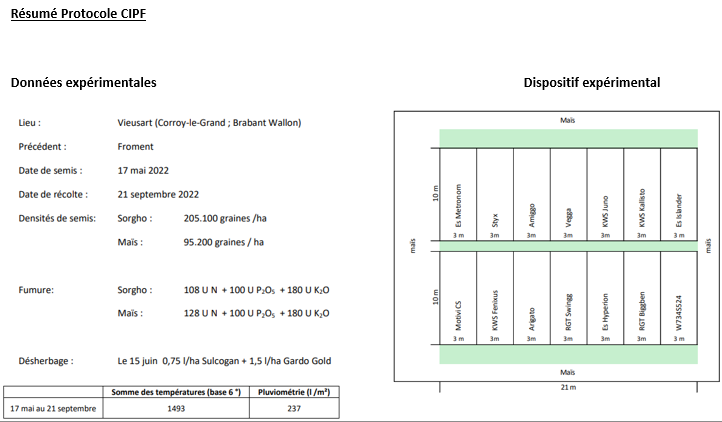
\includegraphics[width=1\textwidth]{Image/protocole CIPF.png}
\caption{Protocole de culture suivi par le CIPF en 2022 \citep{cipf_resultats_2022}}
\end{figure}

\newpage

\newappendix{Solution nutritive de Hoagland}
\label{an:Hoagland}
\begin{table}[ht]
\centering
\caption{Composition de la solution nutritive de Hoagland}
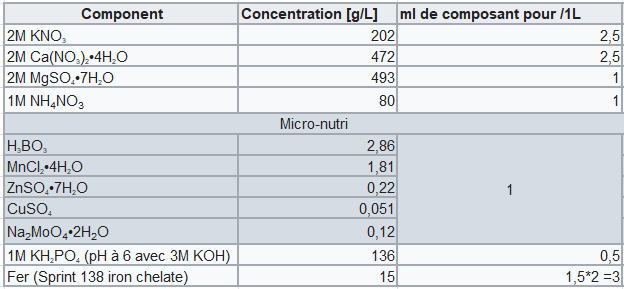
\includegraphics[width=1\textwidth]{Image/hoagland.png}
\end{table}

\newpage

\newappendix{Exemple de tracé de rhizotron}
\label{an:trace}
\begin{figure}[ht]
\centering
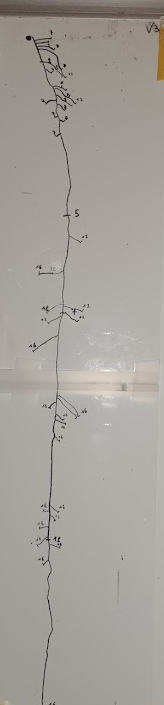
\includegraphics[width=0.235\textwidth]{Image/trace.png}
\caption{Exemple de tracé de rhizotron}
\end{figure}

\newpage

\newappendix{Représentation visuelle d'un fichier RSML}
\label{an:RSML}
\begin{figure}[ht]
\centering
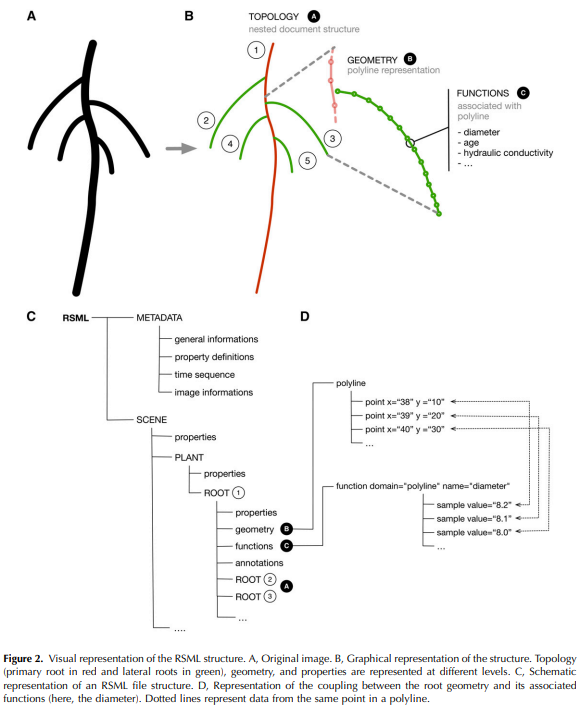
\includegraphics[width=0.8\textwidth]{Image/RSML.png}
\caption{Représentation visuelle d'un fichier RSML provenant de \cite{lobet_root_2015}}
\end{figure}

\newpage

\newappendix{Diagramme ombrothermique culture de Sorgho 2020,2021 et 2022}
\label{an:aerial}
\begin{figure}[ht]
\centering
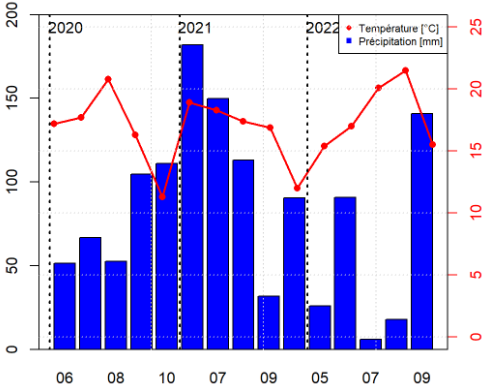
\includegraphics[width=0.8\textwidth]{Image/ombrothermique.png}
\caption{Diagramme ombrothermique des périodes de cultures de sorgho du CIPF}
\end{figure}

\newpage

\newappendix{Estimation monocot}
\label{an:Poaceae}
\begin{figure}[ht]
\centering
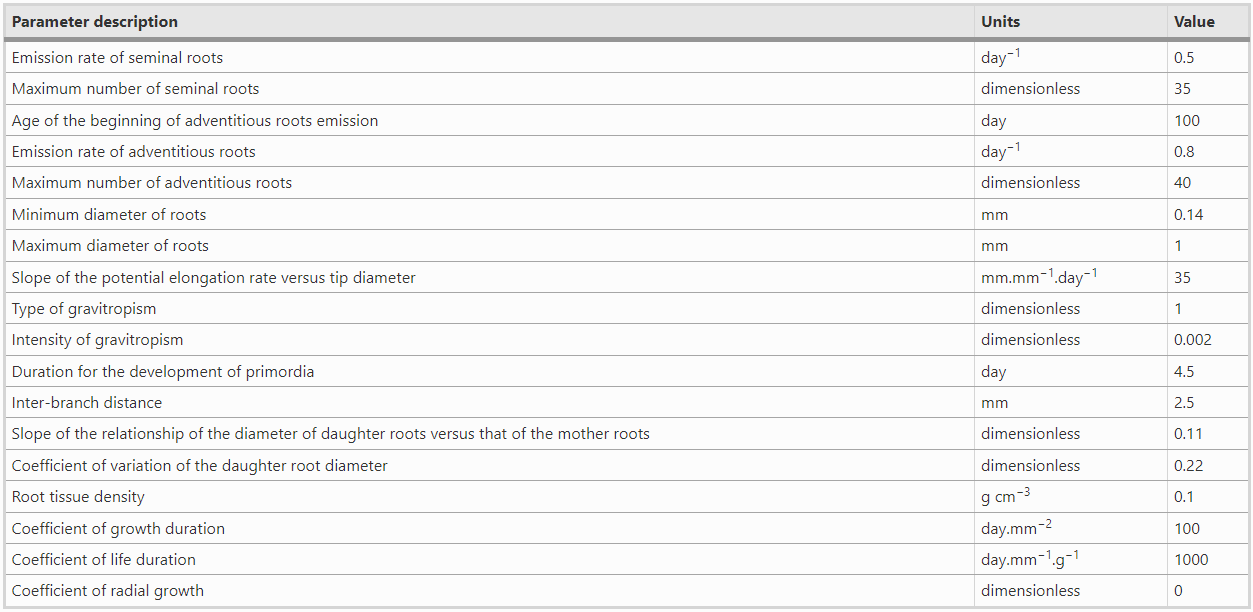
\includegraphics[width=1\textwidth]{Image/parametre Poaceae.png}
\caption{Tableau estimation des paramètres ArchiSimple pour les monocot de \cite{gerard_modelling_2017}}
\end{figure}

\newpage

\newappendix{Dmin}
\label{an:Dmin}
\begin{table}[ht]
\centering
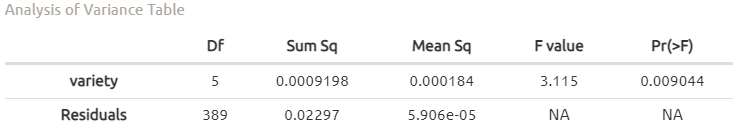
\includegraphics[width=0.65\textwidth]{Image/anova Dmin.png}
\caption{ANOVA du modèle pour estimer Dmin}
\end{table}
\begin{figure}[ht]
\centering
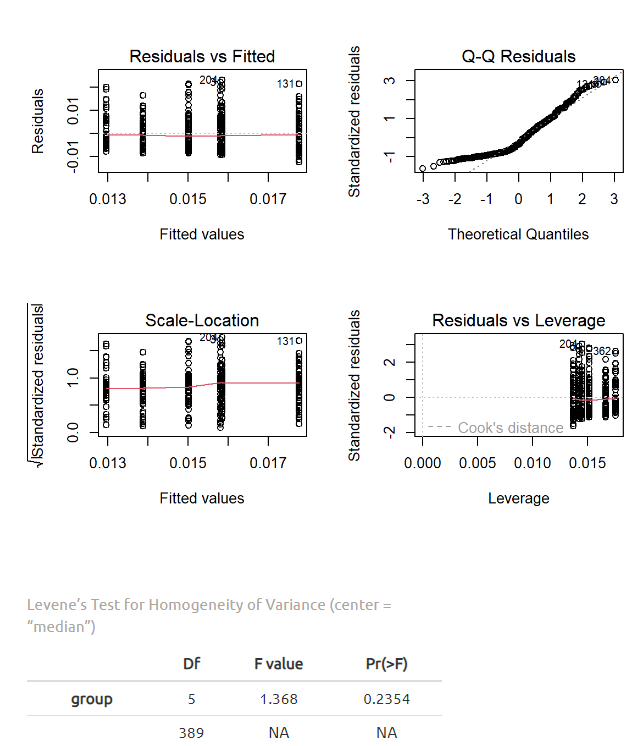
\includegraphics[width=0.65\textwidth]{Image/hypothese Dmin.png}
\caption{Hypothèses Dmin}
\end{figure}
\noindent Indépendance : Assurée par le design et le bon contrôle des conditions expérimentales \\
Normalité : Q-Q plot est OK \\
Egalité des variance : Test de Levene est bon

\newpage

\newappendix{Dmax}
\label{an:Dmax}
\begin{table}[ht]
\centering
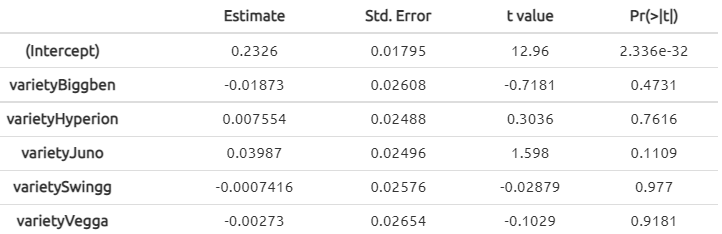
\includegraphics[width=0.6\textwidth]{Image/summary Dmax.png}
\caption{Summary du modèle pour estimer Dmax}
\end{table}
\begin{figure}[ht]
\centering
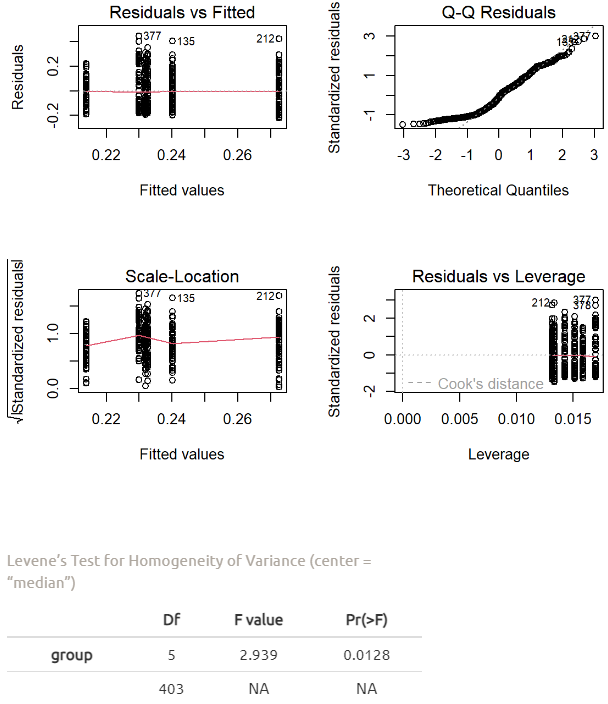
\includegraphics[width=0.6\textwidth]{Image/hypothese Dmax.png}
\caption{Hypothèses Dmax}
\end{figure}
\noindent Indépendance : Assurée par le design et le bon contrôle des conditions expérimentales \\
Normalité : Q-Q plot est OK \\
Egalité des variance : Test de Levene pas bon !

\newpage

\newappendix{Drange}
\label{an:Drange}
\begin{figure}[ht]
\centering
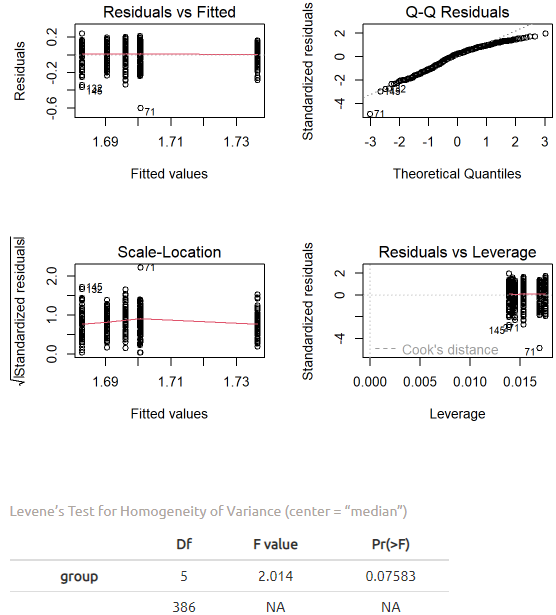
\includegraphics[width=0.6\textwidth]{Image/hypothese Drange.png}
\caption{Hypothèses Drange}
\end{figure}
\noindent Indépendance : Assurée par le design et le bon contrôle des conditions expérimentales \\
Normalité : Q-Q plot est OK \\
Egalité des variance : Test de Levene juste OK !

\newpage

\newappendix{IBD}
\label{an:IBD}
\begin{figure}[ht]
\centering
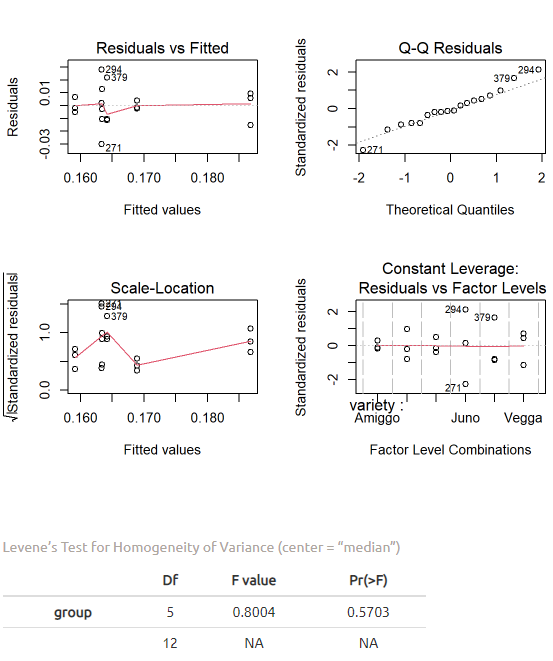
\includegraphics[width=0.4\textwidth]{Image/hypothese IBD}
\caption{Hypothèses IBD}
\end{figure}
\noindent Indépendance : Assurée par le design et le bon contrôle des conditions expérimentales \\
Normalité : Q-Q plot est OK \\
Egalité des variance : Test de Levene juste OK !
\begin{table}[ht]
\centering
\caption{Contrast IBD}
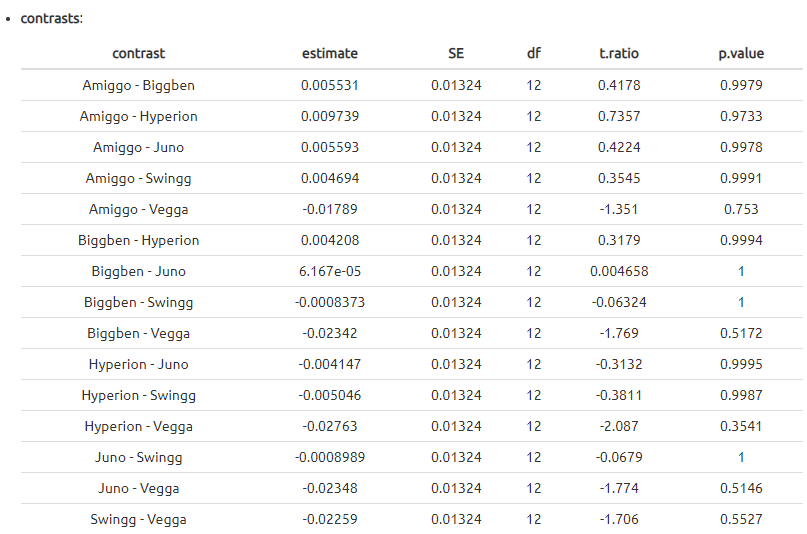
\includegraphics[width=0.5\textwidth]{Image/contrast IBD.png}
\end{table}

\newpage

\newappendix{DIDm}
\label{an:DIDm}
\begin{figure}[ht]
\centering
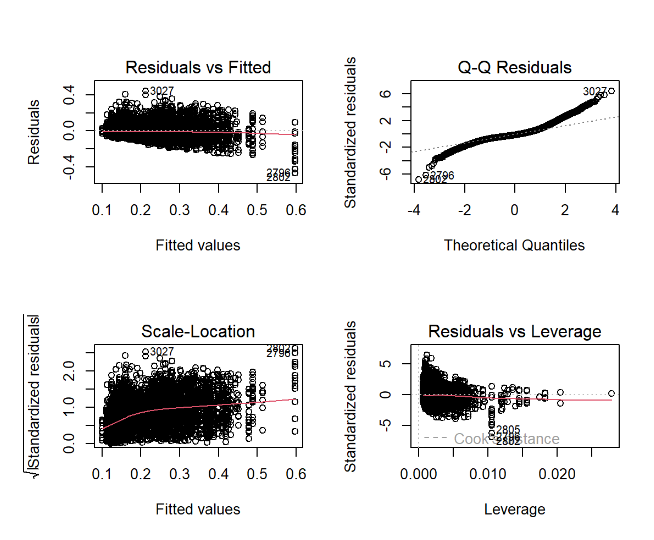
\includegraphics[width=0.6\textwidth]{Image/hypothese DIDm.png}
\caption{Hypothèses DIDm}
\end{figure}
\begin{table}[ht]
\centering
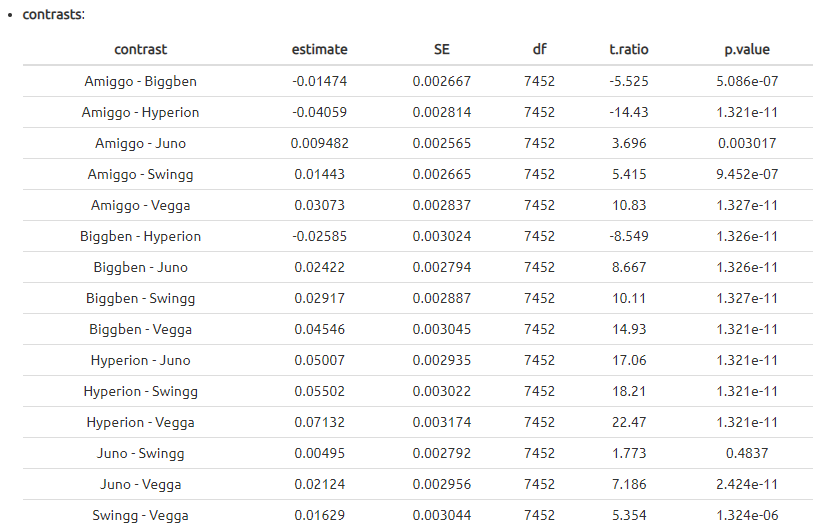
\includegraphics[width=0.6\textwidth]{Image/contrast DIDm.png}
\caption{Contrastes DIDm}
\end{table}

\newpage

\newappendix{CVDD}
\label{an:CVDD}
\begin{figure}[ht]
\centering
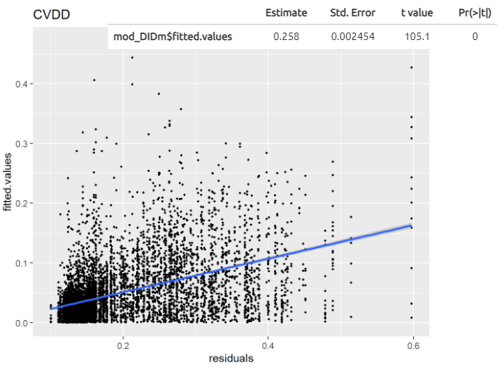
\includegraphics[width=0.55\textwidth]{Image/CVDD.png}
\caption{Graphe et estimation CVDD}
\end{figure}

\newpage

\newappendix{Paramètre maïs}
\label{an:Maize}
\begin{table}[ht]
    \centering
    \caption{Estimation et source des paramètres ArchiSimple pour le maïs}
    \begin{tabular}{c c c}
        Paramètre & Esti & Source \\
        \hline
       simtime & / & / \\
       erSem & 0.5 & \cite{kumar_goyal_how_2021} \\
       dSem & 0.1 & / \cite{pace_analysis_2014} \\
       maxSem & 7 & \cite{kumar_goyal_how_2021} \\
       ageAdv & 7 & \cite{kumar_goyal_how_2021} \\
       distAdv & 30 & / \\
       erAdv & 0.9 & \cite{pages_calibration_2014} adapté \\
       dAdv & 0.3901 & \cite{noauthor_global_2023} \\
       maxAdv & 40 & \cite{pages_calibration_2014} \\
       dmin & 0.14 & \cite{pages_calibration_2014} \\
       dmax & 4.5 & \cite{vanhees_root_2020} \\
       EL & 32.5 & \cite{cahn_relationship_1989} \\
       TrT & 1 & \cite{pages_calibration_2014} \\
       TrInt & 0.01 & \cite{pages_calibration_2014} \\
       PDT & 4.5 & \cite{gerard_modelling_2017} \\
       IPD & 2 & \cite{pages_calibration_2014} \\
       pdmax & 0.8 & / \\
       pdmin & 0 & / \\
       RDM & 0.12 & \cite{pages_calibration_2014} \\
       CVDD & 0.3 & \cite{pages_calibration_2014} \\
       TMD & 0.08 & \cite{pages_calibration_2014} \\
       GDs & 50 & \cite{pages_calibration_2014} \\
       SGC & 0 & \cite{pages_calibration_2014} \\
       LDC & 3000 & \cite{pages_calibration_2014}
    \end{tabular}
\end{table}

\newpage

\newappendix{Diamètre en fonction du noeuds}
\label{an:node_dia}
\begin{figure}[ht]
\centering
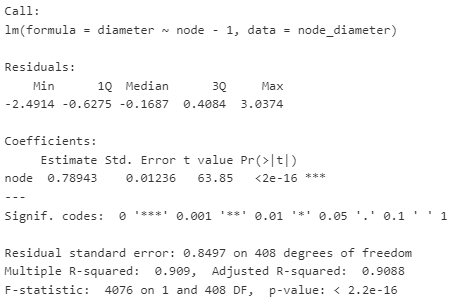
\includegraphics[width=0.7\textwidth]{Image/summary node_dia.png}
\caption{Summary du modèle pour les diamètres en fonction du noeud}
\end{figure}